%----------------------------------------------------------------------------------------
%	PACKAGES AND OTHER DOCUMENT CONFIGURATIONS
%----------------------------------------------------------------------------------------
\documentclass[8pt,x11names]{article} 
\usepackage{ragged2e}
\usepackage{tikz}
\usepackage{graphicx}
\usetikzlibrary{matrix,positioning,calc}


\usepackage[hidelinks]{hyperref}

\pagestyle{empty}

\usepackage{xcolor}     
\usepackage{fontspec} 
\usepackage{fontawesome5}

\usepackage{lmodern}
\renewcommand{\familydefault}{\sfdefault}
\setmonofont{sourcecodepro}

\usepackage{moresize}

\definecolor{claret}{HTML}{820535}   
\definecolor{gunmetal}{HTML}{15212E}     
\definecolor{richblack}{HTML}{080705}
\definecolor{bluish}{HTML}{0B434F}
\definecolor{goldish}{HTML}{8F8414}

%----------------------------------------------------------------------------------------
%	PAGE LAYOUT
%----------------------------------------------------------------------------------------

\usepackage{geometry} % Required for adjusting page dimensions and margins

\geometry{
	paper=letterpaper, % Paper size, letterpaper for US letter size
	top=1.5cm, % Top margin
	bottom=1.5cm, % Bottom margin
	left=2cm, % Left margin
	right=2cm, % Right margin
	headheight=0.75cm, % Header height
	footskip=1cm, % Space from the bottom margin to the baseline of the footer
	headsep=0.5cm, % Space from the top margin to the baseline of the header
	%showframe, % Uncomment to show how the type block is set on the page
}

%----------------------------------------------------------------------------------------
\begin{document}

%----------------------------------------------------------------------------------------
%	TITLE AND CONTACT INFORMATION
%----------------------------------------------------------------------------------------
	
    \begin{tikzpicture}
    
    \matrix[every node/.style={anchor=west,font=\huge}] (name) at (-4,0) {
 	\node{\huge{Lora Johns}}; \\
 % \node{Johns}; \\
 	\node{\color{richblack}\LARGE\textit{data science}}; \\
 	\node{\color{richblack!87}\large\textit{they/them}}; \\
};

\matrix [right = 5cm of name, column 1/.style={anchor=center,color=claret},
         column 2/.style={anchor=west}] (contact) {
%\node{\faMapMarker*};&\node{New York City}; \\
  \node{\faPhone};&\node{203 908 6990}; \\
  \node{\faEnvelope};&\node{{\href{mailto:me@lorajohns.com}{me@lorajohns.com}}}; \\
};

\matrix [right=of contact, column 1/.style={anchor=center,color=claret},
         column 2/.style={anchor=west}] (social) {
  %\node{\faGlobe}; &\node{lorajohns.com}; \\ 
  %\node{\faMedium};&\node{@lorajohns}; \\
  \node{\faGithub}; &\node{{\href{https://www.github.com/lorarjohns}{lorarjohns}}}; \\ 
  \node{\faLinkedin};&\node{{\href{https://www.linkedin.com/in/lora-johns}{lora-johns}}}; \\
};

%----------------------------------------------------------------------------------------
%	INTRODUCTION, SKILLS AND TECHNOLOGIES
%----------------------------------------------------------------------------------------

%----------------------------------------------------------------------------------------
%	ADDITIONAL INFORMATION
%----------------------------------------------------------------------------------------
\node[below=1cm of name,style={anchor=west},inner sep=0pt,text width=10cm] (summary) at (-2,-2){Data science and machine learning generalist with broad \\quantitative and analytic skills and expertise in linguistics, law, and business. Specialist in using alternative data to ask and answer \\creative questions.};

\node[below=4cm of name,font=\large,anchor=west,color=claret!70,inner sep=0pt] (git) at (-3,-1) {GitHub projects};
\matrix [below=0.3cm of git, column 1/.style={anchor=west,color=claret},
         column 2/.style={anchor=west,text width=4cm}, column 3/.style={anchor=west,color=richblack!87,text width=5cm}] {
\node{\faCaretRight};&\node{\href{https://github.com/lorarjohns/nyc_taxi_bigquery}{Hot Tips for Cabbies}};&\node{BigQuery ML on alternative data with SQL}; \\
\node{\faCaretRight};&\node{\href{https://github.com/lorarjohns/SCOTUS}{Topic Modeling the Supreme Court}};&\node{End-to-end unsupervised learning with custom spaCy pipeline}; \\
\node{\faCaretRight};&\node{\href{https://github.com/lorarjohns/cookiecutter_compose}{Docker Compose Cookiecutter}};&\node{Python package for NLP project development}; \\
%\node{\faCaretRight};&\node{\href{https://github.com/lorarjohns/PoliticsLP}{\#StumpTweets}};&\node{Analyzing campaign speeches with Gensim and spaCy}; \\
 };
 
\node[right=5.5cm of git,font=\large,anchor=west,color=claret!70,inner sep=0pt] (prof) {Professional Activities};
\matrix [below=0.3cm of prof, column 1/.style={anchor=west,color=claret},
         column 2/.style={anchor=west,text width=5cm}] {
\node{\faCaretRight};&\node{Correlation One DS4A Summit Presenter 2019}; \\
\node{\faCaretRight};&\node{PyData Diversity Scholar 2019}; \\
\node{\faCaretRight};&\node{PyCon 2020 Program Committee}; \\
\node{\faCaretRight};&\node{Towards Data Science Featured Contributor}; \\
%\node{\faCaretRight};&\node{PyPI Packaging Sprint at DataDog}; \\
%\node{\faCaretRight};&\node{PyGotham Conference, 2019}; \\
%\node{\faCaretRight};&\node{Kaggle Intersection Congestion Competition}; \\
 };
 
 
% image here
\node[below=6cm of git,inner sep=0pt] (gitgraph) at (2,-3.5)
	{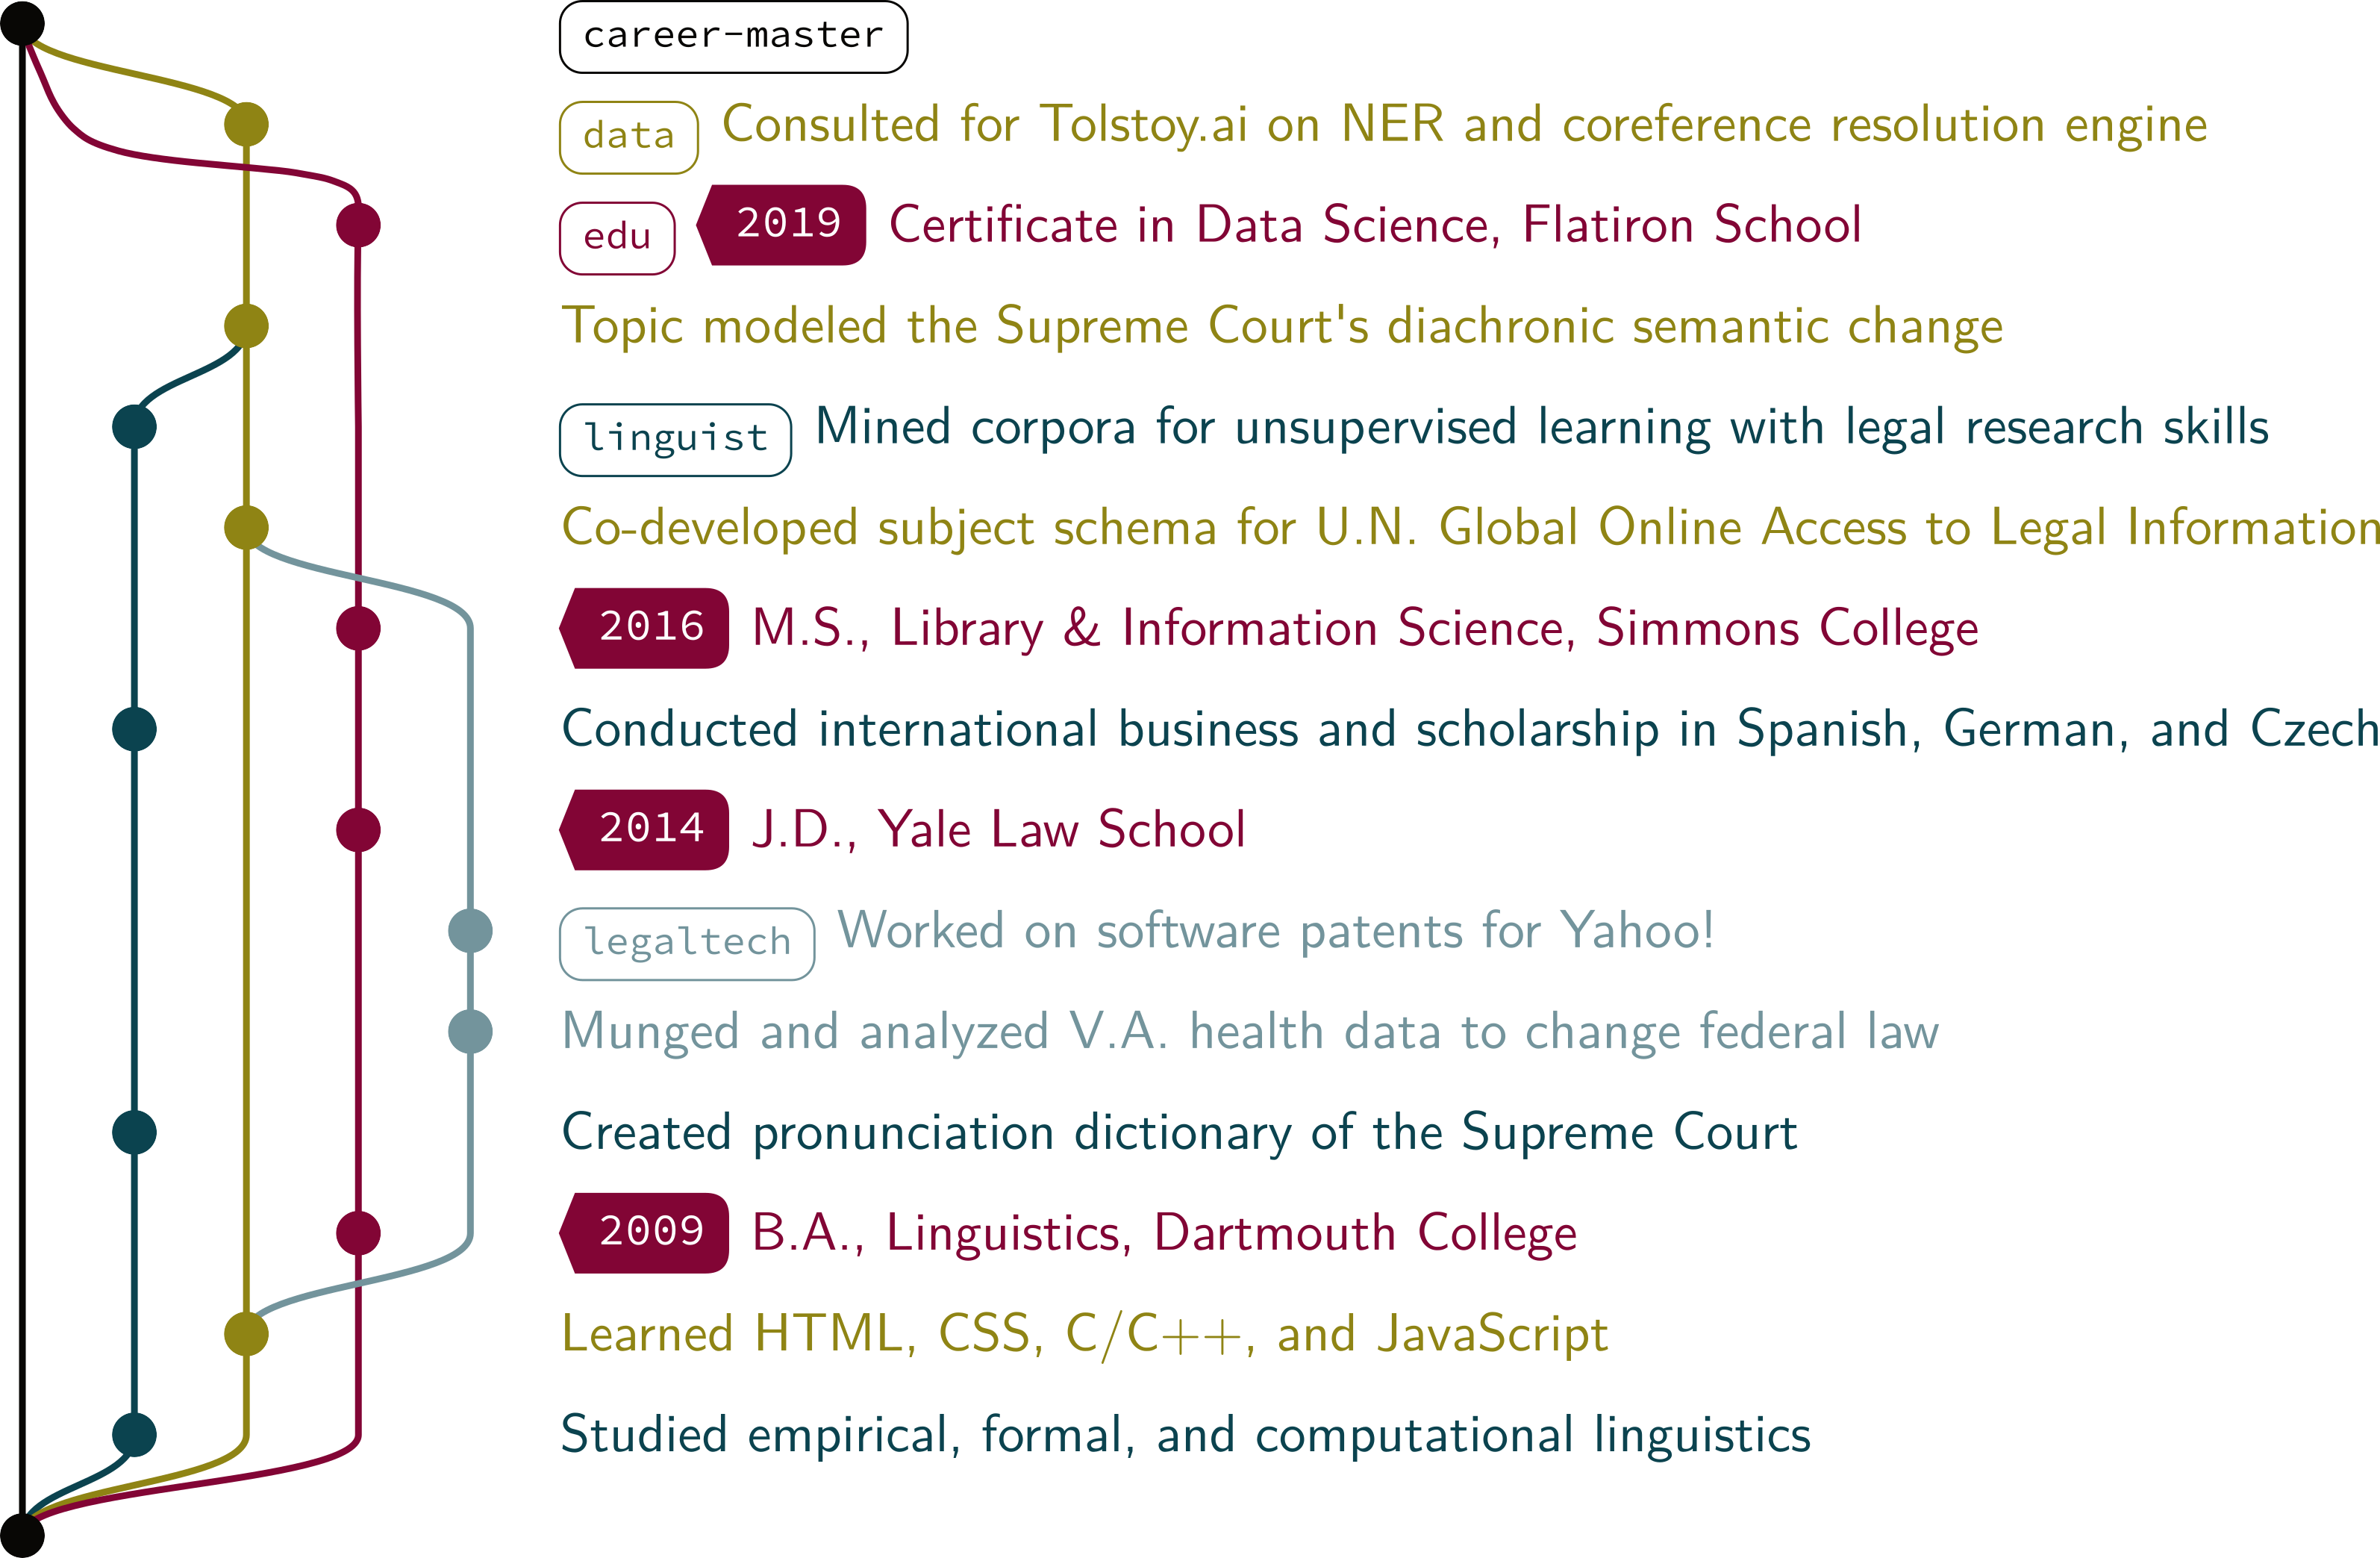
\includegraphics[width=0.75\pagewidth]{../img/compact.png}};

%\node[below=0.1cm of gitgraph,font=\large,anchor=west,color=claret!70,inner sep=0pt] (skills) at (-2,-22) {Skills};
%\matrix [below=0.1cm of skills, column 1/.style={anchor=west,color=claret,text width=0.25cm},column 2/.style={anchor=west,text width=1.25cm},column 3/.style={anchor=west,color=goldish,text width=0.25cm},column 4/.style={anchor=west,text width=1.25cm},column
%	5/.style={anchor=west,color=claret,text width=0.25cm},column
%	6/.style={anchor=west,text width=1.25cm},column
%	7/.style={anchor=west,color=bluish,text width=0.25cm},column
%	8/.style={anchor=west,text width=1.25cm}] {
	%\node{\faRProject};&\node{R};&\node{\faPython};&\node{Python};&\node{\faDatabase};&\node{SQL};&\node{\faCloud};&\node{ ML};\\
	%\node{\faDocker};&\node{Docker};&\node{\faCodeBranch};&\node{GitHub};&\node{\faTerminal};&\node{Bash};&\node{\faLinux};&\node{Linux};\\
 %   };

\node[below=2cm of gitgraph,font=\large,anchor=west,color=claret!70,text width=2cm,inner sep=0pt] (skills) at (-5,-20) {Selected Skills \& Interests};
\matrix [right=0.1cm of skills,column 1/.style={anchor=west,color=claret,text width=1cm},column 2/.style={anchor=west,text width=10cm}]{
\node{\faPython[regular]};&\node{pandas, scikit-learn, numpy, scipy, TensorFlow};\\
\node{\faLinux[regular]};&\node{Linux, bash, C\slash C++\slash Cython};\\
\node{\faRProject[regular]};&\node{\#tidyTuesday R community project};\\
\node{\faTerminal[regular]};&\node{Code sprints, hackathons, or data salons for diversity \& inclusion};\\
};

%----------------------------------------------------------------------------------------

%----------------------------------------------------------------------------------------
%	EXPERIENCE
%----------------------------------------------------------
\end{tikzpicture}
\end{document}